In the map communication pattern each tasks reads and writes to specific data elements in memory.
In its simplicity, the same function or computation is done on each piece of data as seen in \autoref{fig:map}.

\begin{figure}[ht]
	\centering
	\fbox{
		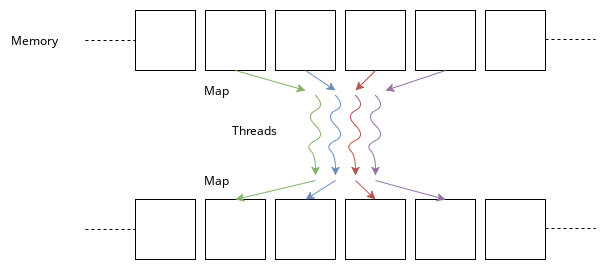
\includegraphics[width=0.6\textwidth]{figs/patterns/parallelmap.png}
	}
	\caption{Map Pattern}
	\label{fig:map}
\end{figure}
This pattern assumes that each task is independent of others.
In the this way there is a one-to-one correspondence between the input and output.
Implementing the map pattern corresponds to that one thread will be executing each task in CUDA.
An example is seen in \autoref{lst:map}.
\FloatBarrier
%TODO: probably move code examples to appendix or include in GitHub
\begin{lstlisting}[language=C,caption={Squaring thread id using map pattern},label=lst:map]
...
__global__ void square(float * d_out, float * d_in){
	int idx = threadIdx.x;
	float f = d_in[idx];
	d_out[idx] = f*f; 	
}

int main(int argc, char ** argv) {
	const int ARRAY_SIZE = 64;
	...
	// generate the input array on the host
	// declare GPU memory pointers, allocate GPU memory, transfer the array to the GPU
	// launch the kernel
	square<<<1, ARRAY_SIZE>>>(d_out, d_in);

	// copy back the result array to the CPU, free device memory
	...
}
\end{lstlisting}


Here the kernel is launched in one block which spawns 64 threads and each thread does the same computation which is to square its thread id and then map each result to memory.